%       \\\ ///      %
%       ( @ @ )      %
% ---o00o.(_).o00o---%
%  Maximilian Bandle %
%  bandle@in.tum.de  %
%  Thesis Template   %
% -------------------%
% \documentclass[draft,headsepline,footsepline,footinclude=false,fontsize=11pt,paper=a4,listof=totoc,bibliography=totoc,BCOR=12mm,DIV=15]{scrbook} % two-sided
\documentclass[headsepline,footsepline,footinclude=false,oneside,fontsize=11pt,paper=a4,listof=totoc,bibliography=totoc]{scrbook} % one-sided

\newcommand*{\getUniversity}{Technische Universität München}
\newcommand*{\getFaculty}{School of Computation, Information and Technology --- Informatics}
% Insert your title here
\newcommand*{\getTitle}{Effects of Linux VFIO for User Space I/O}
\newcommand*{\getTitleGer}{Effekt von Linux VFIO auf User Space E/A}
% Insert your name here
\newcommand*{\getAuthor}{Adrian Simon Würth}
% Type of the document
\newcommand*{\getDoctype}{Bachelor's Thesis in Informatics}
% Choose your supervisor
%\newcommand*{\getSupervisor}{Prof. Alfons Kemper, Ph.D.}
\newcommand*{\getSupervisor}{Prof. Dr. Thomas Neumann}
% \newcommand*{\getSupervisor}{Prof. Dr. Jana Giceva}
% Insert your Advisor
\newcommand*{\getAdvisor}{Simon Ellmann, M.Sc.}
% Official submission date
\newcommand*{\getSubmissionDate}{August 15, 2024}
\newcommand*{\getSubmissionLocation}{Munich}

\PassOptionsToPackage{table,svgnames,dvipsnames}{xcolor}

\usepackage[utf8]{inputenc}
\usepackage[T1]{fontenc}
\usepackage[sc]{mathpazo}
\usepackage[american]{babel}
\usepackage[autostyle]{csquotes}
\usepackage[%
  % backend=biber, % somehow biber did not work properly with latexrun. If you find a solution, feel free to open a merge request
  backend=bibtex,
  url=false,
  style=alphabetic,
  maxnames=4,
  minnames=3,
  maxbibnames=99,
  giveninits,
  uniquename=init]{biblatex}
\usepackage[final]{graphicx}
\usepackage{xcolor}
\usepackage{textcomp}
\usepackage{scrhack} % necessary for listings package
\usepackage[final]{listings}
\usepackage{lstautogobble}
\usepackage{tikz}
\usepackage{booktabs}
\usepackage[labelfont=bf]{caption}
\usepackage[final]{microtype}
\usepackage[final, hidelinks, pdfusetitle]{hyperref} % hidelinks removes colored boxes around references and links
\usepackage{multirow}

\usepackage{setspace}
\usepackage{subcaption}

\hypersetup{
  pdftitle={\getTitle},
  pdfsubject={\getDoctype},
  pdfauthor={\getAuthor},
  pdfkeywords={}
}

\usepackage{float}
\usepackage{algorithm}
\usepackage[noend]{algpseudocode}

\newcommand{\imagePath}[1]{figures/#1}

\bibliography{bibliography}

\setkomafont{disposition}{\normalfont\bfseries} % use serif font for headings
\linespread{1.05} % adjust line spread for mathpazo font

% TUM Colors
\definecolor{TUMblue}{RGB}{0,101,189} % TUMBlau

% 150 Years
\definecolor{TUMgreen}{RGB}{161,191,22} % Gruen
\definecolor{TUMpink}{RGB}{227,130,143} % Rosa
\definecolor{TUMorange}{RGB}{243,145,0} % Orange
\definecolor{TUMbrown}{RGB}{202,171,41} % Senf
\definecolor{TUMblueLight}{RGB}{91,197,242}  % Hellblau

% 150 Years (Light)
\definecolor{TUMlightGreen}{RGB}{188,207,30} % Gruen
\definecolor{TUMlightPink}{RGB}{242,144,149} % Rosa
\definecolor{TUMlightOrange}{RGB}{247,166,0} % Orange
\definecolor{TUMlightBrown}{RGB}{232,200,55} % Senf
\definecolor{TUMlightBlueLight}{RGB}{146,212,241} % Hellblau

% Settings for algorithm
\algnewcommand\algorithmicforeach{\textbf{for each}}
\algdef{S}[FOR]{ForEach}[1]{\algorithmicforeach\ #1\ \algorithmicdo}

% Settings for lstlistings
\lstset{%
  basicstyle=\ttfamily,
  columns=fullflexible,
  autogobble,
  keywordstyle=\bfseries\color{MediumBlue},
  stringstyle=\color{DarkGreen}
}

\usepackage{amsmath}

% Define auto scale
\makeatletter
\def\ScaleIfNeeded{%
  \ifdim\Gin@nat@width>\textwidth
    \textwidth
  \else
    \Gin@nat@width
  \fi
}
\makeatother

% % If Draft 
% \usepackage{ifdraft}

% % Show labels in draft
% \usepackage[inline]{showlabels}
% \ifdraft{
%   \showlabels[\color{TUMblue}]{cite}
%   \showlabels[\color{TUMorange}]{ref}
% }{}

% \usepackage{showkeys}

% % Draft Footer 
% \ifdraft{
%   \usepackage[draft=false]{scrlayer-scrpage} % Use this as final to avoid rulers
%   \cfoot*{Draft Version (\today)}
% }{}

% FixMe Notes and Warnings
\usepackage{fixme}
\fxsetup{theme=color,author=}

% Chapter Symbols for progress
\def\draftEmpty{\rlap{\protect\makebox[-3cm]{\color{red}$\circ$}}}
\def\draftProgress{\rlap{\protect\makebox[-3cm]{\color{yellow}$\circ$}}}
\def\draftDone{\rlap{\protect\makebox[-3cm]{\color{green}$\circ$}}}

% TUM Logo
% This is tumlogo.tex
%
% Neues TUM-Logo in TeX
%   by G. Teege, 19.10.89
% Benutzung:
%   Am Anfang des Dokuments (TeX oder LaTeX):
%     \input tumlogo
%   Dann beliebig oft:
%     \TUM{<breite>}
%   bzw.
%     \oTUM{<breite>}
%   \TUM setzt das Logo mit der Breite <breite> und der entsprechenden Hoehe.
%   <breite> muss eine <dimen> sein. \oTUM erzeugt eine "outline"-Version
%   des Logos, d.h. weiss mit schwarzem Rand. Bei \TUM ist es ganz schwarz.
%   \oTUM entspricht damit der offiziellen Version des Logos.
%   Das Logo kann wie ein einzelnes Zeichen verwendet werden.
%   Beispiel:
%     Dies ist das TUM-Logo: \oTUM{1cm}.
%
\def\TUM#1{%
\dimen1=#1\dimen1=.1143\dimen1%
\dimen2=#1\dimen2=.419\dimen2%
\dimen3=#1\dimen3=.0857\dimen3%
\dimen4=\dimen1\advance\dimen4 by\dimen2%
\setbox0=\vbox{\hrule width\dimen3 height\dimen1 depth0pt\vskip\dimen2}%
\setbox1=\vbox{\hrule width\dimen1 height\dimen4 depth0pt}%
\setbox2=\vbox{\hrule width\dimen3 height\dimen1 depth0pt}%
\setbox3=\hbox{\copy0\copy1\copy0\copy1\box2\copy1\copy0\copy1\box0\box1}%
\leavevmode\vbox{\box3}}
%
\def\oTUM#1{%
\dimen1=#1\dimen1=.1143\dimen1%
\dimen2=#1\dimen2=.419\dimen2%
\dimen3=#1\dimen3=.0857\dimen3%
\dimen0=#1\dimen0=.018\dimen0%
\dimen4=\dimen1\advance\dimen4 by-\dimen0%
\setbox1=\vbox{\hrule width\dimen0 height\dimen4 depth0pt}%
\advance\dimen4 by\dimen2%
\setbox8=\vbox{\hrule width\dimen0 height\dimen4 depth0pt}%
\advance\dimen4 by-\dimen2\advance\dimen4 by-\dimen0%
\setbox4=\vbox{\hrule width\dimen4 height\dimen0 depth0pt}%
\advance\dimen4 by\dimen1\advance\dimen4 by\dimen3%
\setbox6=\vbox{\hrule width\dimen4 height\dimen0 depth0pt}%
\advance\dimen4 by\dimen3\advance\dimen4 by\dimen0%
\setbox9=\vbox{\hrule width\dimen4 height\dimen0 depth0pt}%
\advance\dimen4 by\dimen1%
\setbox7=\vbox{\hrule width\dimen4 height\dimen0 depth0pt}%
\dimen4=\dimen3%
\setbox5=\vbox{\hrule width\dimen4 height\dimen0 depth0pt}%
\advance\dimen4 by-\dimen0%
\setbox2=\vbox{\hrule width\dimen4 height\dimen0 depth0pt}%
\dimen4=\dimen2\advance\dimen4 by\dimen0%
\setbox3=\vbox{\hrule width\dimen0 height\dimen4 depth0pt}%
\setbox0=\vbox{\hbox{\box9\lower\dimen2\copy3\lower\dimen2\copy5%
\lower\dimen2\copy3\box7}\kern-\dimen2\nointerlineskip%
\hbox{\raise\dimen2\box1\raise\dimen2\box2\copy3\copy4\copy3%
\raise\dimen2\copy5\copy3\box6\copy3\raise\dimen2\copy5\copy3\copy4\copy3%
\raise\dimen2\box5\box3\box4\box8}}%
\leavevmode\box0}
% End of tumlogo.tex




\begin{document}

% Set page numbering to avoid  "destination with the same identifier has been already used" warning for cover page.
% (see https://en.wikibooks.org/wiki/LaTeX/Hyperlinks#Problems_with_Links_and_Pages).
\pagenumbering{alph}
\begin{titlepage}
  % HACK for two-sided documents: ignore binding correction for cover page.
  % Adapted from Markus Kohm's KOMA-Script titlepage=firstiscover handling.
  % See http://mirrors.ctan.org/macros/latex/contrib/koma-script/scrkernel-title.dtx,
  % \maketitle macro.
  \oddsidemargin=\evensidemargin\relax
  \textwidth=\dimexpr\paperwidth-2\evensidemargin-2in\relax
  \hsize=\textwidth\relax

  \centering
  \oTUM{38mm}

  \vspace{5mm}
  \begin{spacing}{1.55}
    {\huge\MakeUppercase{\getFaculty{}}}\\
  \end{spacing}

  \vspace{5mm}
  {\large\MakeUppercase{\getUniversity{}}}\\

  \vspace{20mm}
  {\Large \getDoctype{}}

  \vspace{15mm}
  {\huge\bfseries \getTitle{}}

  \vspace{15mm}
  {\LARGE \getAuthor{}}

  % \ifdraft{Draft (\today)}{}

  \IfFileExists{include/logos/faculty.pdf}{%
    \vspace{20mm}
    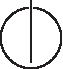
\includegraphics[height=20mm]{include/logos/faculty.pdf}
  }{}
\end{titlepage}


\frontmatter{}

\begin{titlepage}
  \centering

  \oTUM{38mm}

  \vspace{5mm}
  \begin{spacing}{1.55}
    {\huge\MakeUppercase{\getFaculty{}}}\\
  \end{spacing}

  \vspace{5mm}
  {\large\MakeUppercase{\getUniversity{}}}\\

  \vspace{20mm}
  {\Large \getDoctype{}}

  \vspace{15mm}
  {\huge\bfseries \getTitle{}}

  \vspace{10mm}
  {\huge\bfseries \getTitleGer{}}

  \vspace{10mm}
  \begin{tabular}{l l}
    Author:          & \getAuthor{}         \\
    Supervisor:      & \getSupervisor{}     \\
    Advisor:         & \getAdvisor{}        \\
    Submission Date: & \getSubmissionDate{} \\
    % \ifdraft{Version: & \today ~(Draft)\\}{}
  \end{tabular}

  \IfFileExists{include/logos/faculty.pdf}{%
    \vfill{}
    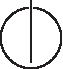
\includegraphics[height=20mm]{include/logos/faculty.pdf}
  }{}
\end{titlepage}
\cleardoublepage{}

\thispagestyle{empty}
\vspace*{0.8\textheight}
\noindent
I confirm that this \MakeLowercase{\getDoctype{}} is my own work and I have documented all sources and material used.

\vspace{15mm}
\noindent
\getSubmissionLocation{}, \today \hspace{50mm} \getAuthor{}

\cleardoublepage{}

% \phantomsection{}
\addcontentsline{toc}{chapter}{Acknowledgments}
\thispagestyle{empty}

\vspace*{20mm}

\begin{center}
{\usekomafont{section} Acknowledgments}
\end{center}

\vspace{10mm}

% Please DONT use all the titles in the Acks and also not the Makros
I would like to express my gratitude to my advisor \getAdvisor{} and my supervisor \getSupervisor{} for the opportunity to work on this interesting topic.

Furthermore, I would like to thank Max for the thesis template. 

Many people, especially my friends have made valuable suggestions on my thesis. Without your ideas and corrections, the thesis would not be as good as it is now. Thanks to my roommates for proofreading and providing ideas throughout the whole process of writing. Thanks to my apartment for letting me live in it. You get the idea.

This section is completely optional and you may also structure is as you like. Writing it in german is also fine.


\cleardoublepage{}

\chapter{Abstract}

We present a framework for students to bootstrap your final thesis. The primary goal of this template is to improve the quality of the thesis by avoiding typical mistakes. Our framework focuses on the basic thesis structure, which is mostly applicable, and helps you to immediately start writing. The first step is that the student writes down what he did so far, and performs some changes to this structure, yielding a thesis with notes and a rough plan how to write it up. The second step is to transform your notes into sentences, yielding a first draft. A template is the first step to the final thesis. In contrast to writing a thesis from scratch, our approach gives you a scaffold and helps you focusing on the important parts. We also show how to plot your data and describe your experiments. We present experimental results showing the perfect final thesis in the end.

As you might already have noticed, the abstract is the first, and sometimes only part the reader notices.
Thus it's crucial to summarize your work while motivating the reader here.
To help you with formulating we provide a basic structure to just fill the gaps.
Afterward, you can and should reformulate it to add your personal touch to it.

[...] present [...] for [...] to [...]. The primary goal of [...] is to improve [...] by avoiding [...] . Our framework focuses on [...], which is [...] , and is [...]. The first [...] , and performs [...], yielding [...]. The second [...] where [...], and yields [...]. [...] is the first [...]. In contrast [...], our approach [...]. We also show how [...]. We present experimental results showing [...].
 

\chapter{Kurzfassung}

In case you are not speaking german, you are free to drop the german abstract.

Dies ist der einzige Teil der Arbeit auf deutsch. 
Die Kurzfassung ist optional.
Sie erfüllt den gleichen Teil wie der englische Abstract, ist aber wahrscheinlich ein bisschen verständlicher, wenn ihr eure Arbeit daheim zeigt.
\microtypesetup{protrusion=false}
\tableofcontents{}
\listoffixmes{}
\microtypesetup{protrusion=true}
\mainmatter{}

\chapter{Introduction}\label{c:introduction}

During his speech "Null Reference: The Billion Dollar Mistake" in 2009, Tony Hoare, a renowned computer scientist, well known for the invention of Quick-sort, proposed the idea of how null pointers are the reason for at least a billion dollars in damages \cite{billiondollarmistake}. This quote could not be more important than at this time. In July 2024, Microsoft devices faced what has been described as the "most spectacular IT meltdown the world has ever seen" \cite{bloombergmeltdown}. This meltdown affected 8.5 million Microsoft Windows devices and severely impacted public institutions, including critical infrastructure like hospitals and airports \cite{bloomberg8milliondevices}. In the root cause analysis paper by Crowdstrike, the cybersecurity company that deployed the faulty code, it was revealed that inproper compile time validation and missing runtime array bounds checks were a big part of the error \cite{crowdstrikerca}.

The damage that can be done by a single ring 0 driver like Crowdstrike's Falcon software shows how critical it is to ensure memory safety. By using Rust, a memory-safe yet highly performant programming language with a restrictive compiler, we could drastically improve security and memory safety. We can witness Rust's influence on the systems development community since even the Linux kernel, which has been using C for almost 30 years without accepting any other languages like C++, now allows Rust code in its codebase \cite{linuxrustpull}.

However, it's also important to consider Rusts safety limits. While using Rust for a driver improves the overall safety of the process while not compensating on performance, direct memory and I/O operations have to be implemented in an unsafe way. A userspace driver using physical DMA addresses enables a device to practically have full access to the memory and potentially do detrimental I/O operations. Malicious firmware attacks are a rising threat.
To enforce safety at the device level, we need to make use of the IOMMU, a safe way of doing direct memory accesses. The IOMMU acts as a layer of isolation between devices and the CPU. By using virtual addresses, the IOMMU provides a bigger virtual address space and enforce memory access rights \cite{OLS2007}.

The primary goal of this thesis is to examine how the IOMMU impacts performance in the context of userspace I/O.
We demonstrate this by implementing IOMMU support on vroom, a NVMe driver written in Rust \cite{vroom}, and comparing it to using physical addresses. We use the Linux framework VFIO to implement the IOMMU functionality, which has the additional benefit of enabling the driver to run without root privileges. Additionally, we will be looking at IOMMUFD, a modern replacement for VFIO's IOMMU API.

\chapter{Building Blocks}

This chapter outlines the building blocks of your work.
It may mean describing what has already be done by others or you reimplementing other aproaches.

We are giving you some hints on writing english academic texts here.
\chapter{My awesome stuff}

This is your main chapter. It should be named after your index structure, or central message.

Here we show sth about draft and todo stuff.
\chapter{Evaluation}
Give some introduction why you are doing these measurements.
Also an overview to allow the reader to find fast what he wants to read.

In general focus when describing on the why and implications.
Just putting plots there and describing is the easy part and does not give the reader insights beyond the plots.
You have to collect the clues and show what happens in the background to explain the development.

Here we evaluate different plotting frameworks to give you an alternative and show you some differences. This is continued in the discussion.

\section{Setup}
State the machines you are using the methods and the compiler if its system level.
Otherwise this section should tell all the steps necessary to reproduce your measurements.

Wollte eig nen barplot, lineplot und noch was mit log scale in allen dreien zeigen und jeweils was es speziell macht. 

\section{Matplotlib}

\section{ggplot}

\section{Seaborn}

\chapter{Discussion}
\chapter{Conclusions}\label{c:c}

% Thesis contribution #1 Overview + AKI
This template gives a brief overview of thesis writing. It has a examplary structure to serve as gantry.
Furthermore we show how to plot using matplotlib, seaborn and ggplot.

% Evaluation #2 ACT
ACT was tested for a spatially disjoint workload and outperforms FAST C++ by several orders of a magnitude. 

\paragraph{Future Work}


In conclusion, this thesis uses novel approaches to lay the foundation for spatio-textual data processing on modern hardware. The presented optimizations to the AKI reach the same level as other state-of-the-art indexes. Spatio-textual ACT provides superior performance for disjoint workloads. 


%\appendix{}
%\chapter{Implementation}\label{c:code}

%\begin{table}[htpb]
%    \centering
%    \begin{tabular}{r|l}
%        \textbf{\#} & \textbf{Category} \\
%        \hline
%\textbf{1} & Restaurants \\
%\textbf{2} & Food \\
%\textbf{3} & Nightlife \\
%\textbf{4} & Shopping \\
%\textbf{5} & Bars \\
%\textbf{6} & German \\
%\textbf{7} & Event Planning \& Services \\
%\textbf{8} & Cafes \\
%\textbf{9} & Coffee \& Tea \\
%\textbf{10} & Italian \\
%\textbf{11} & Hotels \& Travel \\
%\textbf{12} & Swabian \\
%\textbf{13} & Hotels \\
%\textbf{14} & Arts \& Entertainment \\
%\textbf{15} & Active Life \\
%\textbf{16} & Fashion \\
%\textbf{17} & Pizza \\
%\textbf{18} & Specialty Food \\
%\textbf{19} & Wine Bars \\
%\textbf{20} & International \\
%\textbf{21} & Fast Food \\
%\textbf{22} & Beer Garden \\
%\textbf{23} & Grocery \\
%\textbf{24} & Caterers \\
%\textbf{25} & Bakeries \\
%\textbf{26} & Pubs \\
%\textbf{27} & Cocktail Bars \\
%\textbf{28} & Burgers \\
%\textbf{29} & Music \& Video \\
%\textbf{30} & Books \\
%\textbf{31} & Mags \\
%\textbf{32} & Mediterranean \\
%\textbf{33} & Bistros \\
%\textbf{34} & Delicatessen \\
%\textbf{35} & Public Services \& Government \\
%\textbf{36} & Greek \\
%\textbf{37} & Lounges \\
%\textbf{38} & Breakfast \& Brunch \\
%\textbf{39} & Dance Clubs \\
%\textbf{40} & Beer \\
%\textbf{41} & Wine \& Spirits \\
%\textbf{42} & Music Venues \\
%\textbf{43} & Steakhouses \\
%\textbf{44} & Vegetarian \\
%\textbf{45} & French \\
%\textbf{46} & Venues \& Event Spaces \\
%\textbf{47} & Landmarks \& Historical Buildings \\
%\textbf{48} & Seafood \\
%\textbf{49} & Sports Clubs \\
%\textbf{50} & Party \& Event Planning \\
%\textbf{51} & Salad \\
%        \end{tabular}
%    \caption[Top 10 Categories in Stuttgart]{Top 10 Categories in Stuttgart}
%    \label{t:data:cities}
%\end{table}

\microtypesetup{protrusion=false}

\listoffigures{}
\listoftables{}
\lstlistoflistings{}

\microtypesetup{protrusion=true}

% Bibliographie Test
\printbibliography{}

\end{document}
